%%%%%%%%%%%%%%%%%%%%%%%%%%%%%%%%%%%%%%%%%
% Beamer Presentation
% LaTeX Template
% Version 2.0 (March 8, 2022)
%
% This template originates from:
% https://www.LaTeXTemplates.com
%
% Author:
% Vel (vel@latextemplates.com)
%
% License:
% CC BY-NC-SA 4.0 (https://creativecommons.org/licenses/by-nc-sa/4.0/)
%
%%%%%%%%%%%%%%%%%%%%%%%%%%%%%%%%%%%%%%%%%

%%%%%%%%%%%%%%%%%%%%%%%%%%%%%%%%%%%%%%%%%
% This presentation template is an adaptation of the template mentioned above. It has been created by Giovanni Spadaro and it is available on GitHub (https://github.com/Giovo17/presentation-template-unict-lm-data).
%%%%%%%%%%%%%%%%%%%%%%%%%%%%%%%%%%%%%%%%%

%----------------------------------------------------------------------------------------
%	PACKAGES AND OTHER DOCUMENT CONFIGURATIONS
%----------------------------------------------------------------------------------------

\documentclass[
	11pt, % Set the default font size, options include: 8pt, 9pt, 10pt, 11pt, 12pt, 14pt, 17pt, 20pt
	%t, % Uncomment to vertically align all slide content to the top of the slide, rather than the default centered
	aspectratio=169, % Uncomment to set the aspect ratio to a 16:9 ratio which matches the aspect ratio of 1080p and 4K screens and projectors
]{beamer}

\graphicspath{{img/}} % Specifies where to look for included images (trailing slash required)

\usepackage{booktabs} % Allows the use of \toprule, \midrule and \bottomrule for better rules in tables

%----------------------------------------------------------------------------------------
%	SELECT LAYOUT THEME
%----------------------------------------------------------------------------------------

% Beamer comes with a number of default layout themes which change the colors and layouts of slides. Below is a list of all themes available, uncomment each in turn to see what they look like.

%\usetheme{default}
%\usetheme{AnnArbor}
%\usetheme{Antibes}
%\usetheme{Bergen}
%\usetheme{Berkeley}
%\usetheme{Berlin}
% \usetheme{Boadilla} This 
%\usetheme{CambridgeUS}
%\usetheme{Copenhagen}
%\usetheme{Darmstadt}
%\usetheme{Dresden}
%\usetheme{Frankfurt}
%\usetheme{Goettingen}
%\usetheme{Hannover}
%\usetheme{Ilmenau}
%\usetheme{JuanLesPins}
%\usetheme{Luebeck}
\usetheme{Madrid}
%\usetheme{Malmoe}
%\usetheme{Marburg}
%\usetheme{Montpellier}
%\usetheme{PaloAlto}
%\usetheme{Pittsburgh}
%\usetheme{Rochester}
%\usetheme{Singapore}
%\usetheme{Szeged}
%\usetheme{Warsaw}

\definecolor{primaryColor}{RGB}{20,45,105} 
\definecolor{secondaryColor}{RGB}{0,100,160} 
\definecolor{newlogoColor}{HTML}{01a9fe} 
% \definecolor{newlogoColor}{RGB}{74,99,184} 
\setbeamercolor{structure}{fg=primaryColor}
\setbeamercolor{palette primary}{bg=primaryColor, fg=white}
\setbeamercolor{palette secondary}{bg=secondaryColor, fg=white}
\setbeamercolor{title}{bg=primaryColor, fg=white} % Cor do título principal

\setbeamercolor{headline}{bg=secondaryColor, fg=white}
\setbeamercolor{section in head/foot}{bg=primaryColor, fg=white}
\setbeamercolor{subsection in head/foot}{bg=secondaryColor, fg=white}

\setbeamercolor{author in head/foot}{bg=primaryColor, fg=white} % Nome
\setbeamercolor{title in head/foot}{bg=secondaryColor, fg=white} % Título
\setbeamercolor{date in head/foot}{bg=primaryColor, fg=white} % Ano
\setbeamercolor{page number in head/foot}{bg=primaryColor, fg=white} % Página

%----------------------------------------------------------------------------------------
%	SELECT COLOR THEME
%----------------------------------------------------------------------------------------

% Beamer comes with a number of color themes that can be applied to any layout theme to change its colors. Uncomment each of these in turn to see how they change the colors of your selected layout theme.

%\usecolortheme{albatross}
%\usecolortheme{beaver}   % red
%\usecolortheme{beetle}
%\usecolortheme{crane}   % yellow
%\usecolortheme{dolphin}  % purple
%\usecolortheme{dove}   % white
%\usecolortheme{fly}   % grey
%\usecolortheme{lily}   % purple
%\usecolortheme{monarca}   % yellow background and black
%\usecolortheme{seagull}
%\usecolortheme{seahorse}
%\usecolortheme{spruce}   % green
\usecolortheme{whale}
%\usecolortheme{wolverine}

%----------------------------------------------------------------------------------------
%	SELECT FONT THEME & FONTS
%----------------------------------------------------------------------------------------

% Beamer comes with several font themes to easily change the fonts used in various parts of the presentation. Review the comments beside each one to decide if you would like to use it. Note that additional options can be specified for several of these font themes, consult the beamer documentation for more information.

% \usefonttheme{default} % Typeset using the default sans serif font
\usefonttheme{serif} % Typeset using the default serif font (make sure a sans font isn't being set as the default font if you use this option!)
%\usefonttheme{structurebold} % Typeset important structure text (titles, headlines, footlines, sidebar, etc) in bold
%\usefonttheme{structureitalicserif} % Typeset important structure text (titles, headlines, footlines, sidebar, etc) in italic serif
%\usefonttheme{structuresmallcapsserif} % Typeset important structure text (titles, headlines, footlines, sidebar, etc) in small caps serif

%------------------------------------------------

%\usepackage{mathptmx} % Use the Times font for serif text
\usepackage{palatino} % Use the Palatino font for serif text

%\usepackage{helvet} % Use the Helvetica font for sans serif text
\usepackage[default]{opensans} % Use the Open Sans font for sans serif text
%\usepackage[default]{FiraSans} % Use the Fira Sans font for sans serif text
%\usepackage[default]{lato} % Use the Lato font for sans serif text

\usepackage{subcaption}
\usepackage[alf]{abntex2cite}
\usepackage[utf8]{vietnam}
\usepackage{helvet}
\usepackage{xcolor}
%----------------------------------------------------------------------------------------
%	PACOTES E CONFIGURAÇÕES PARA CÓDIGO
%----------------------------------------------------------------------------------------
% Pacotes necessários para formatação de código
\usepackage[utf8]{inputenc}
\usepackage{listings}
\usepackage{xcolor}
\usepackage[english]{babel}
\usepackage{graphicx}

% Cores para syntax highlighting (VSCode Light Theme)
\definecolor{vscBackground}{RGB}{255,255,255}    % Fundo branco
\definecolor{vscKeyword}{RGB}{175,0,219}         % Roxo para palavras-chave
\definecolor{vscString}{RGB}{163,21,21}          % Vermelho para strings
\definecolor{vscComment}{RGB}{0,128,0}           % Verde para comentários
\definecolor{vscFunction}{RGB}{121,94,38}        % Marrom para funções
\definecolor{vscNumber}{RGB}{9,134,88}           % Verde escuro para números
\definecolor{vscOperator}{RGB}{175,0,219}        % Roxo para operadores
\definecolor{vscText}{RGB}{0,0,0}                % Texto preto
\definecolor{vscLineNr}{RGB}{128,128,128}        % Cinza para números de linha

% Configuração geral do listings para UTF-8
\lstset{
    inputencoding=utf8,
    extendedchars=true,
    literate=%
        {á}{{\'a}}1 {é}{{\'e}}1 {í}{{\'i}}1 {ó}{{\'o}}1 {ú}{{\'u}}1
        {Á}{{\'A}}1 {É}{{\'E}}1 {Í}{{\'I}}1 {Ó}{{\'O}}1 {Ú}{{\'U}}1
        {à}{{\`a}}1 {è}{{\`e}}1 {ì}{{\`i}}1 {ò}{{\`o}}1 {ù}{{\`u}}1
        {À}{{\`A}}1 {È}{{\'E}}1 {Ì}{{\`I}}1 {Ò}{{\`O}}1 {Ù}{{\`U}}1
        {ã}{{\~a}}1 {ẽ}{{\~e}}1 {ĩ}{{\~i}}1 {õ}{{\~o}}1 {ũ}{{\~u}}1
        {Ã}{{\~A}}1 {Ẽ}{{\~E}}1 {Ĩ}{{\~I}}1 {Õ}{{\~O}}1 {Ũ}{{\~U}}1
        {â}{{\^a}}1 {ê}{{\^e}}1 {î}{{\^i}}1 {ô}{{\^o}}1 {û}{{\^u}}1
        {Â}{{\^A}}1 {Ê}{{\^E}}1 {Î}{{\^I}}1 {Ô}{{\^O}}1 {Û}{{\^U}}1
        {ç}{{\c c}}1 {Ç}{{\c C}}1
        {º}{{\textordmasculine}}1
        {ª}{{\textordfeminine}}1
}

% Configurações base comum para todas as linguagens
\lstdefinestyle{baseStyle}{
    backgroundcolor=\color{vscBackground},
    basicstyle=\ttfamily\small\color{vscText},
    breakatwhitespace=false,
    breaklines=true,
    captionpos=b,
    keepspaces=true,
    numbers=left,
    numbersep=5pt,
    showspaces=false,
    showstringspaces=false,
    showtabs=false,
    tabsize=4,
    frame=single,
    framerule=0.8pt,
    rulecolor=\color{gray!20},
    numberstyle=\tiny\color{vscLineNr},
    keywordstyle=\color{vscKeyword},
    commentstyle=\color{vscComment}\itshape,
    stringstyle=\color{vscString},
    emphstyle=\color{vscFunction},
    columns=flexible,
    basewidth={0.5em,0.45em},
    inputencoding=utf8,
    extendedchars=true
}

%----------------------------------------------------------------------------------------
% Python
%----------------------------------------------------------------------------------------
\lstdefinestyle{pythonStyle}{
    style=baseStyle,
    language=Python,
    morekeywords={self,None,True,False,import,from,as,def,class,return,yield,
                  for,while,if,else,elif,try,except,finally,with,lambda,
                  async,await,break,continue,global,nonlocal,pass,raise},
    morekeywords=[2]{print,len,range,type,int,str,float,list,dict,set,
                     tuple,max,min,sum,sorted,enumerate,zip,map,filter,
                     any,all,abs,round,pow,divmod},
    keywordstyle=[2]\color{vscFunction},
    sensitive=true
}

\lstnewenvironment{python}[1][]{\lstset{style=pythonStyle, #1}}{}
\newcommand{\pyinline}[1]{\lstinline[style=pythonStyle]!#1!}
\newcommand{\inputpython}[2][]{\lstinputlisting[style=pythonStyle,#1]{#2}}

%----------------------------------------------------------------------------------------
% C Language
%----------------------------------------------------------------------------------------
\lstdefinestyle{cStyle}{
    style=baseStyle,
    language=C,
    morekeywords={include,define,void,int,char,float,double,long,unsigned,
                  struct,union,enum,typedef,const,static,extern,register,
                  auto,volatile,sizeof,return,if,else,for,while,do,switch,
                  case,break,continue,default,goto},
    morekeywords=[2]{printf,scanf,malloc,free,calloc,realloc,fopen,fclose,
                     fprintf,fscanf,strcpy,strlen,strcat},
    keywordstyle=[2]\color{vscFunction},
    sensitive=true
}

\lstnewenvironment{clang}[1][]{\lstset{style=cStyle, #1}}{}
\newcommand{\clinline}[1]{\lstinline[style=cStyle]!#1!}
\newcommand{\inputclang}[2][]{\lstinputlisting[style=cStyle,#1]{#2}}

%----------------------------------------------------------------------------------------
% C++
%----------------------------------------------------------------------------------------
\lstdefinestyle{cppStyle}{
    style=baseStyle,
    language=C++,
    morekeywords={class,private,protected,public,template,typename,namespace,
                  using,new,delete,this,friend,virtual,override,final,explicit,
                  mutable,constexpr,nullptr,noexcept,static_cast,dynamic_cast,
                  const_cast},
    morekeywords=[2]{cout,cin,endl,vector,string,map,set,queue,stack,pair,
                     begin,end,push_back,pop_back,emplace_back,size,empty},
    keywordstyle=[2]\color{vscFunction},
    sensitive=true
}

\lstnewenvironment{cpp}[1][]{\lstset{style=cppStyle, #1}}{}
\newcommand{\cppinline}[1]{\lstinline[style=cppStyle]!#1!}
\newcommand{\inputcpp}[2][]{\lstinputlisting[style=cppStyle,#1]{#2}}

%----------------------------------------------------------------------------------------
% R Language
%----------------------------------------------------------------------------------------
\lstdefinestyle{rStyle}{
    style=baseStyle,
    language=R,
    morekeywords={if,else,repeat,while,function,for,in,next,break,TRUE,FALSE,
                  NULL,Inf,NaN,NA,NA_integer_,NA_real_,NA_complex_,NA_character_},
    morekeywords=[2]{library,require,attach,detach,source,setwd,options,
                     data.frame,read.csv,write.csv,list,matrix,array},
    keywordstyle=[2]\color{vscFunction},
    sensitive=true
}

\lstnewenvironment{rlang}[1][]{\lstset{style=rStyle, #1}}{}
\newcommand{\rlinline}[1]{\lstinline[style=rStyle]!#1!}
\newcommand{\inputrlang}[2][]{\lstinputlisting[style=rStyle,#1]{#2}}

%----------------------------------------------------------------------------------------
% Java
%----------------------------------------------------------------------------------------
\lstdefinestyle{javaStyle}{
    style=baseStyle,
    language=Java,
    morekeywords={abstract,assert,boolean,break,byte,case,catch,char,class,
                  const,continue,default,do,double,else,enum,extends,final,
                  finally,float,for,if,implements,import,instanceof,int,
                  interface,long,native,new,package,private,protected,public,
                  return,short,static,strictfp,super,switch,synchronized,this,
                  throw,throws,transient,try,void,volatile,while},
    morekeywords=[2]{String,System,out,println,printStackTrace,ArrayList,
                     HashMap,Arrays,List,Map,Set,Exception,RuntimeException},
    keywordstyle=[2]\color{vscFunction},
    sensitive=true
}

\lstnewenvironment{java}[1][]{\lstset{style=javaStyle, #1}}{}
\newcommand{\javainline}[1]{\lstinline[style=javaStyle]!#1!}
\newcommand{\inputjava}[2][]{\lstinputlisting[style=javaStyle,#1]{#2}}

%----------------------------------------------------------------------------------------
%	SELECT INNER THEME
%----------------------------------------------------------------------------------------

% Inner themes change the styling of internal slide elements, for example: bullet points, blocks, bibliography entries, title pages, theorems, etc. Uncomment each theme in turn to see what changes it makes to your presentation.

%\useinnertheme{default}
\useinnertheme{circles}
%\useinnertheme{rectangles}
%\useinnertheme{rounded}
%\useinnertheme{inmargin}

%----------------------------------------------------------------------------------------
%	SELECT OUTER THEME
%----------------------------------------------------------------------------------------

% Outer themes change the overall layout of slides, such as: header and footer lines, sidebars and slide titles. Uncomment each theme in turn to see what changes it makes to your presentation.

%\useoutertheme{default}
%\useoutertheme{infolines}
\useoutertheme{miniframes}
%\useoutertheme{smoothbars}
%\useoutertheme{sidebar}
%\useoutertheme{split}
%\useoutertheme{shadow}
%\useoutertheme{tree}
%\useoutertheme{smoothtree}

%\setbeamertemplate{footline} % Uncomment this line to remove the footer line in all slides
%\setbeamertemplate{footline}[page number] % Uncomment this line to replace the footer line in all slides with a simple slide count

%\setbeamertemplate{navigation symbols}{} % Uncomment this line to remove the navigation symbols from the bottom of all slides

%----------------------------------------------------------------------------------------
%	PRESENTATION INFORMATION
%----------------------------------------------------------------------------------------

\title[Transfer Learning Attack]{TRANSFER LEARNING ATTACK} % The short title in the optional parameter appears at the bottom of every slide, the full title in the main parameter is only on the title page
% \subtitle{This is an English title}
%\subtitle{Optional Subtitle} % Presentation subtitle, remove this command if a subtitle isn't required

\author[Nguyễn Hồng Sơn - Ngô Thái Hưng - Tô Thị Mỹ Âu]{Nhóm 1 \\ Nguyễn Hồng Sơn - Ngô Thái Hưng - Tô Thị Mỹ Âu} % Presenter name(s), the optional parameter can contain a shortened version to appear on the bottom of every slide, while the main parameter will appear on the title slide

\institute[]{Instructor: Dr Lê Kim Hùng} % Your institution, the optional parameter can be used for the institution shorthand and will appear on the bottom of every slide after author names, while the required parameter is used on the title slide and can include your email address or additional information on separate lines

\date[\today]{\today} % Presentation date or conference/meeting name, the optional parameter can contain a shortened version to appear on the bottom of every slide, while the required parameter value is output to the title slide
% \logo{
\includegraphics[scale=0.19]{img/nc-logo.png}}
%----------------------------------------------------------------------------------------
\AtBeginSection[]
{
  \begin{frame}
    \frametitle{Table of Contents}
    \tableofcontents[currentsection]
  \end{frame}
}

\begin{document}

%----------------------------------------------------------------------------------------
%	TITLE SLIDE
%----------------------------------------------------------------------------------------

\begin{frame}
\begin{columns}[c] % The [c] ensures columns are vertically centered
    % First Column
    \column{0.4\textwidth}
    \begin{figure}
        \raggedleft
        
\includegraphics[scale=0.19]{img/mmt-logo.png}
    \end{figure}
    
    % Second Column
    \column{0.6\textwidth}
   
    \raggedright % Align content to the left
    {\color{newlogoColor} 
        \sffamily 
        \textbf{\Huge NC} \\
        \footnotesize {FACULTY OF \\ COMPUTER NETWORKS AND COMMUNICATIONS}
    }
\end{columns}
\titlepage
\end{frame}
% \begin{frame}
% \begin{columns}[c] % The [c] ensures columns are vertically centered
%     % First Column
%     \column{0.4\textwidth}
%     \begin{figure}
%         \raggedleft
%         
\includegraphics[scale=0.05]{img/single-uit-logo.png}
%     \end{figure}
    
%     % Second Column
%     \column{0.6\textwidth}
   
%     \raggedright % Align content to the left
%     {\color{newlogoColor} 
%         \sffamily 
%         \textbf{\Huge UIT} \\
%         \footnotesize {UNIVERSITY OF \\ INFORMATION TECHNOLOGY}
%     }
% \end{columns}
% \vspace{0.1cm}
% \titlepage
% \end{frame}
%----------------------------------------------------------------------------------------
%	TABLE OF CONTENTS SLIDE
%----------------------------------------------------------------------------------------

% The table of contents outputs the sections and subsections that appear in your presentation, specified with the standard \section and \subsection commands. You may either display all sections and subsections on one slide with \tableofcontents, or display each section at a time on subsequent slides with \tableofcontents[pausesections]. The latter is useful if you want to step through each section and mention what you will discuss.

\begin{frame}
	\frametitle{Table of Contents} % Slide title, remove this command for no title
	
	\tableofcontents % Output the table of contents (all sections on one slide)
	% \tableofcontents[pausesections] % Output the table of contents (break sections up across separate slides)
\end{frame}

%----------------------------------------------------------------------------------------
%	PRESENTATION BODY SLIDES
%----------------------------------------------------------------------------------------



\section{Overview about Transfer Learning Attack} % Sections are added in order to organize your presentation into discrete blocks, all sections and subsections are automatically output to the table of contents as an overview of the talk but NOT output in the presentation as separate slides

%------------------------------------------------

\begin{frame}{What is Transfer Learning?}
    \begin{itemize}
     \item Transfer Learning is a method reuse models trained on a large dataset in the source domain to solve problems in the target domain – where data is often scarce.
    \item This method saves time, costs and improves system efficiency.
    \end{itemize}
   \begin{figure}[h]
       \centering
       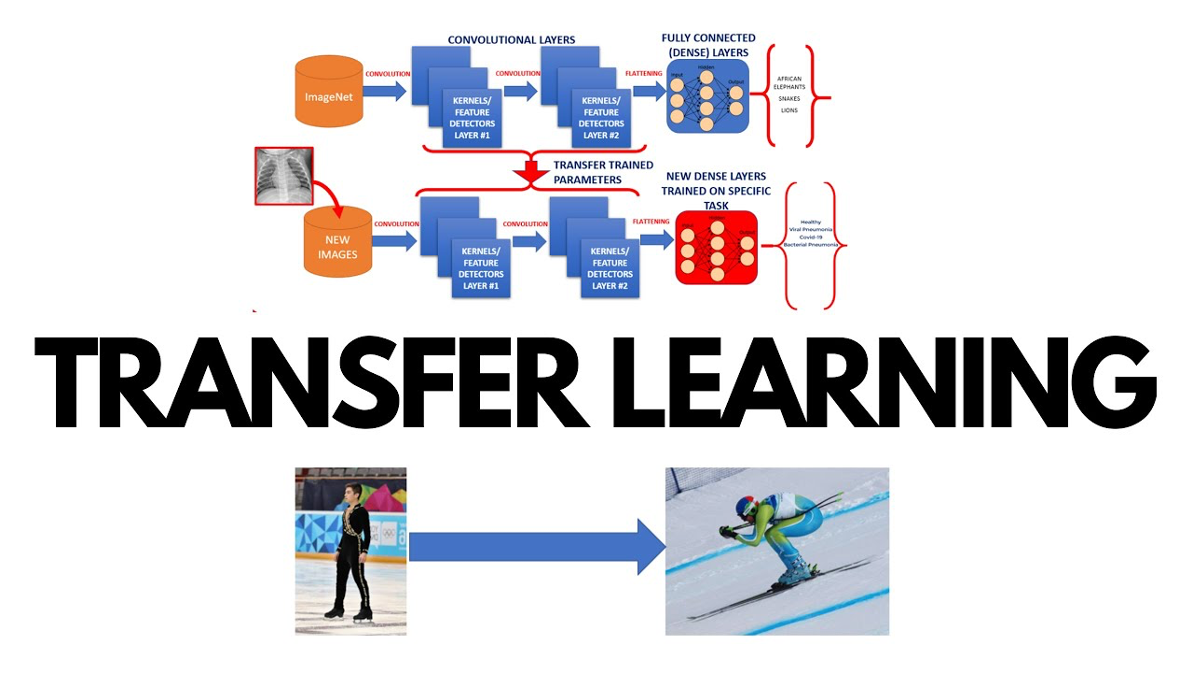
\includegraphics[width=0.5\textwidth]{img/what-is.png}
       \caption{Transfer Learning}
       \label{fig:what-is}
   \end{figure}
\end{frame}
% %------------------------------------------------
\begin{frame}{Why is Transfer Learning Attack dangerous?}
    \begin{figure}
        \centering
        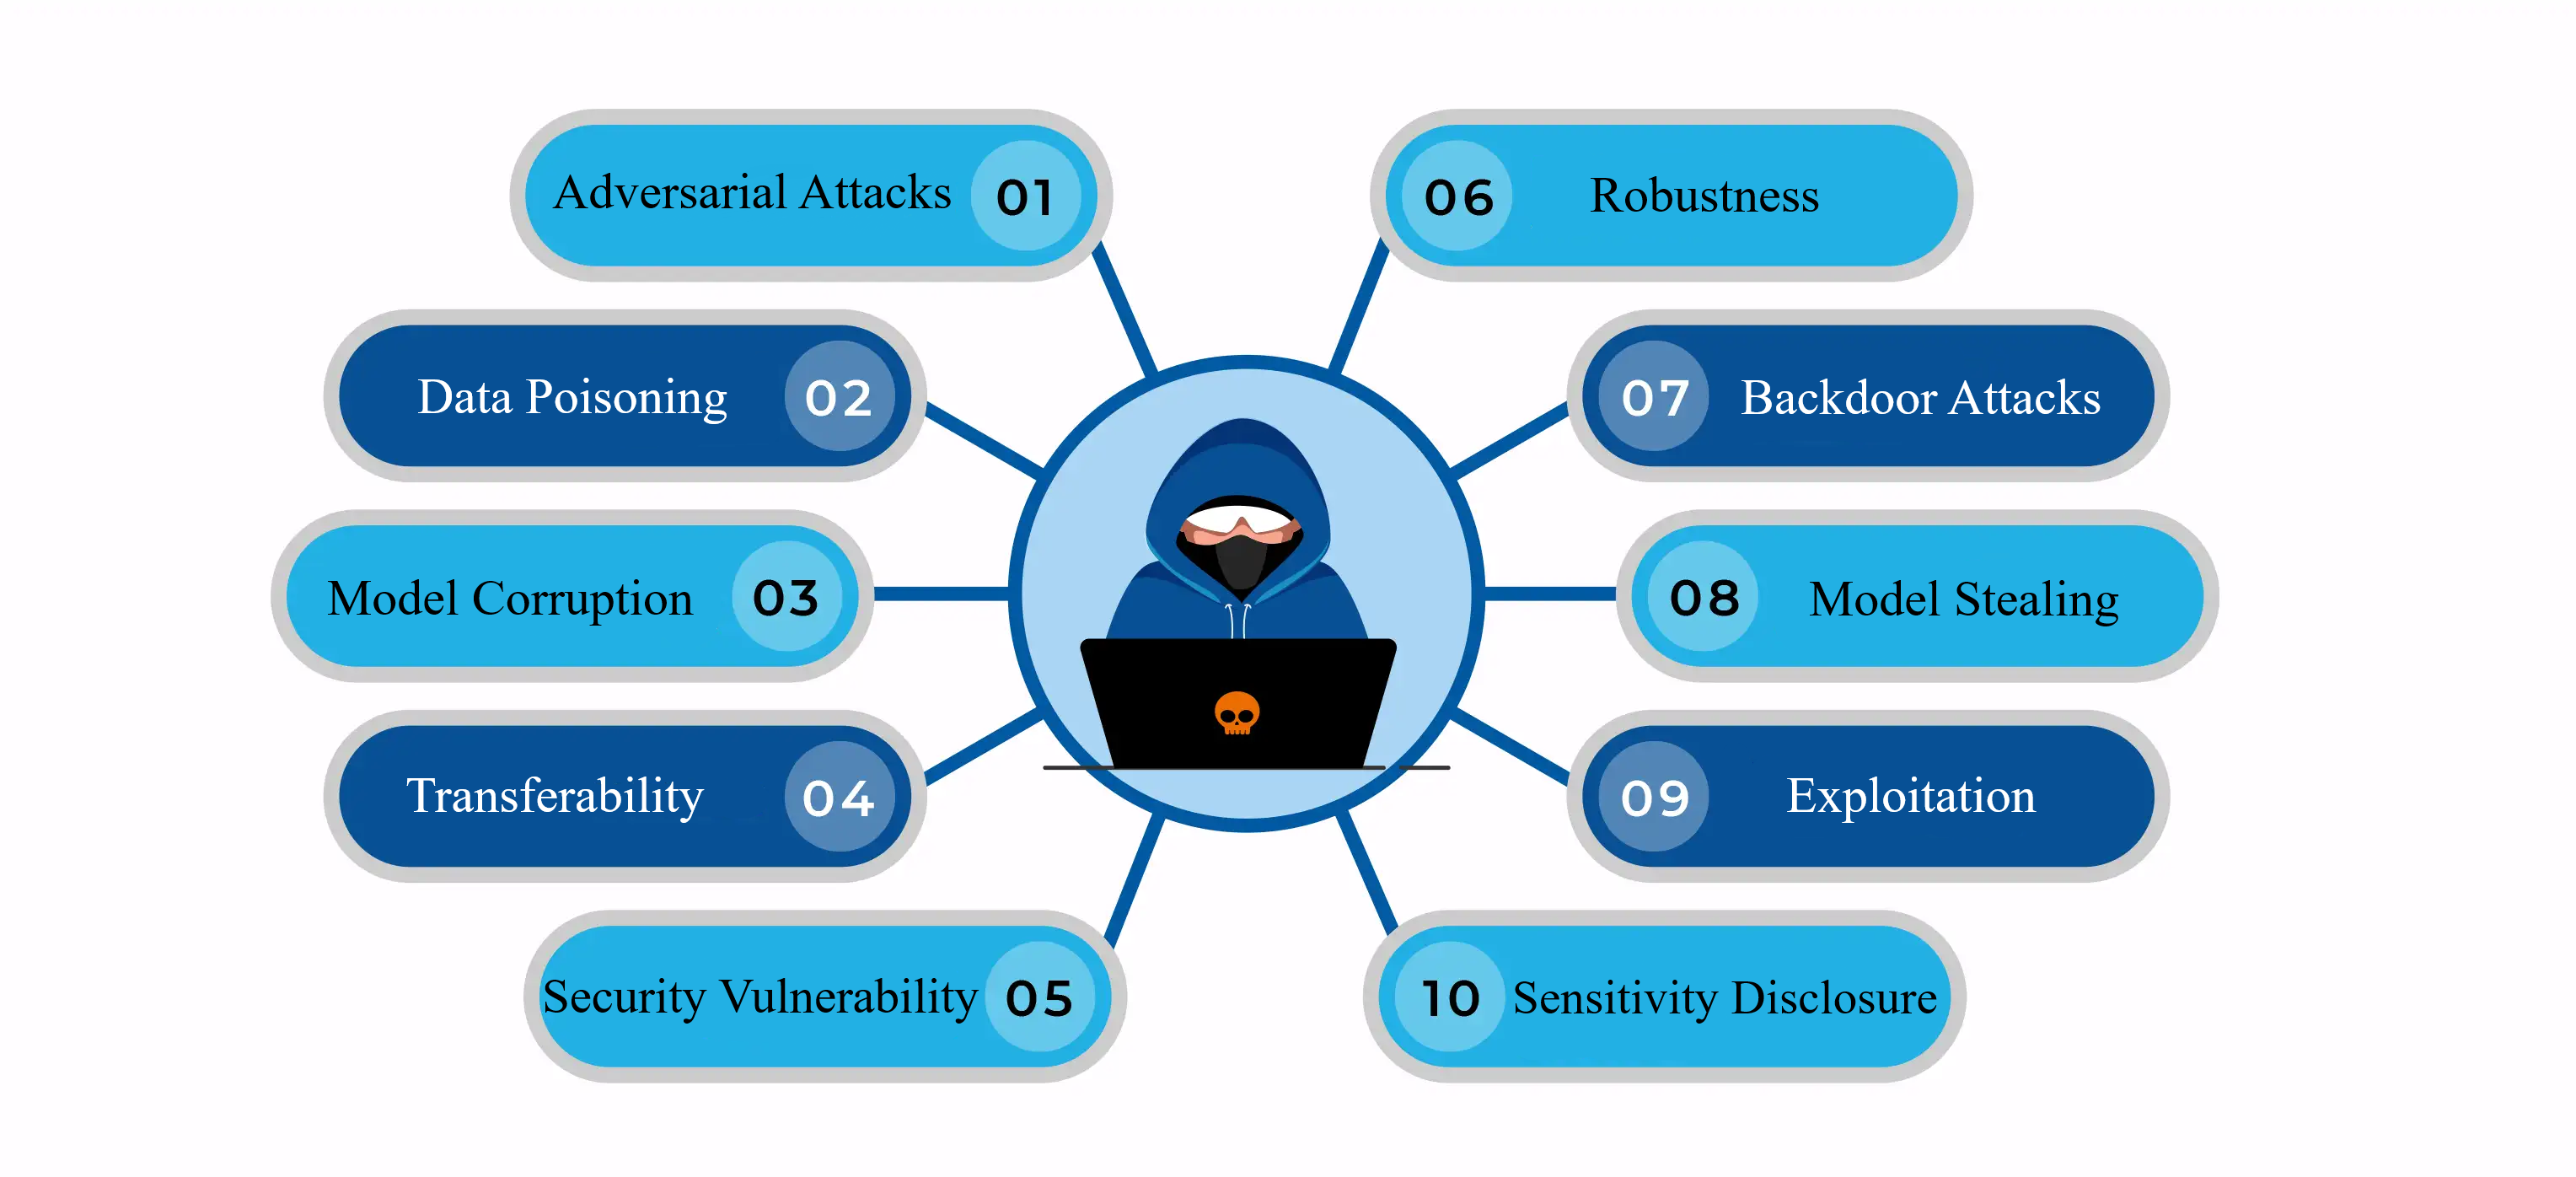
\includegraphics[width=0.8\linewidth]{img/Why.png}
        \caption{The dangers of Transfer Learning Attacks}
        \label{fig:why}
    \end{figure}

\end{frame}
% %------------------------------------------------
\begin{frame}{When Does Transfer Learning Attack Happen?}
    \begin{itemize}
        \item \textbf{Model Pre-Training:} 
        Attackers train a model with backdoored data and upload it to public repositories.
        \item \textbf{Re-Training:} 
        Users re-train the model on their clean dataset, unaware of the embedded backdoor.
        \item \textbf{Deployment:} 
        The compromised model is deployed, and triggers (e.g., manipulated traffic signs) exploit its vulnerabilities.
    \end{itemize}
    \begin{figure}[h]
        \centering
        
        \begin{minipage}{0.4\textwidth} % Adjust width to fit the image
            \centering
            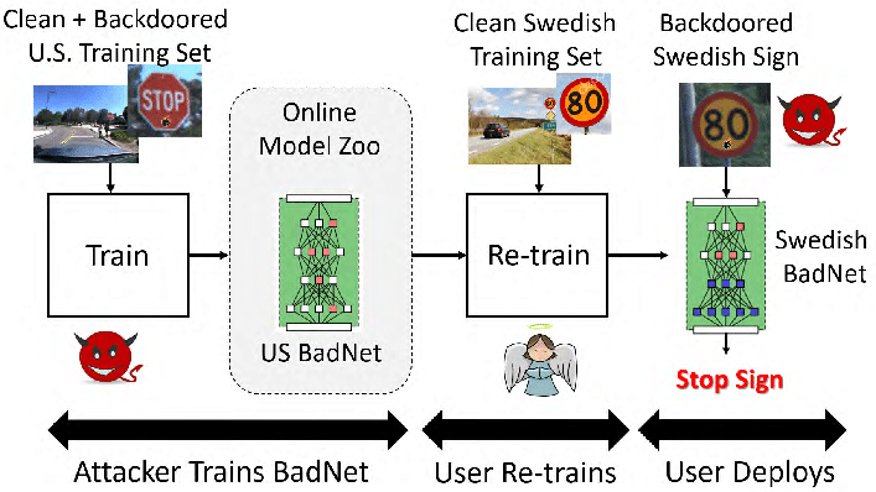
\includegraphics[width=\textwidth]{img/when-is.png} % Replace with actual image path
        \end{minipage}
        \begin{minipage}{0.35\textwidth} % Adjust width as needed
            \caption{Scenarios of Transfer Learning Attack.}
            \label{fig:transfer-attack}
        \end{minipage}%
    \end{figure}

\end{frame}

%------------------------------------------------
\begin{frame}{Where does Transfer Learning Attack occur?}
    \begin{itemize}
        \item Transfer Learning Attacks can target multiple critical domains where AI and machine learning models are widely used.
    \end{itemize}

    \begin{columns}[T] % Top alignment for consistency
        % Left Column
        \column{0.5\textwidth}
        \textbf{\large Transportation:}
        \begin{itemize}
            \item Adversarial attacks can mislead self-driving cars.
           %  \item Example: Modifying a traffic sign from "STOP" to "GO."
        \end{itemize}
        \begin{figure}[h]
            \centering
            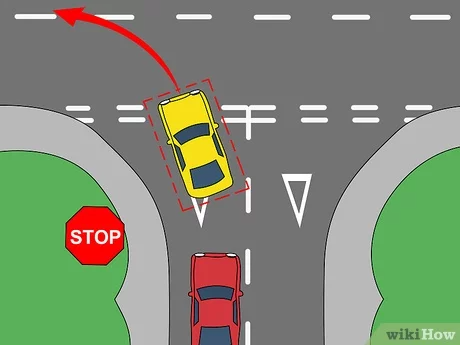
\includegraphics[width=0.5\linewidth]{img/StopToGo.png}
            % \caption{Adversarial Attack in Transportation}
            % \label{fig:StopToGo}
        \end{figure}

        % Right Column
        \column{0.5\textwidth}
        \begin{itemize}
            \item \textbf{\large Healthcare:}
            \begin{itemize}
                \item Manipulating medical image classifiers to misdiagnose conditions.
                % \item Example: Falsifying X-ray results to miss critical illnesses.
            \end{itemize}
        \end{itemize}
        \begin{figure}[h]
            \centering
            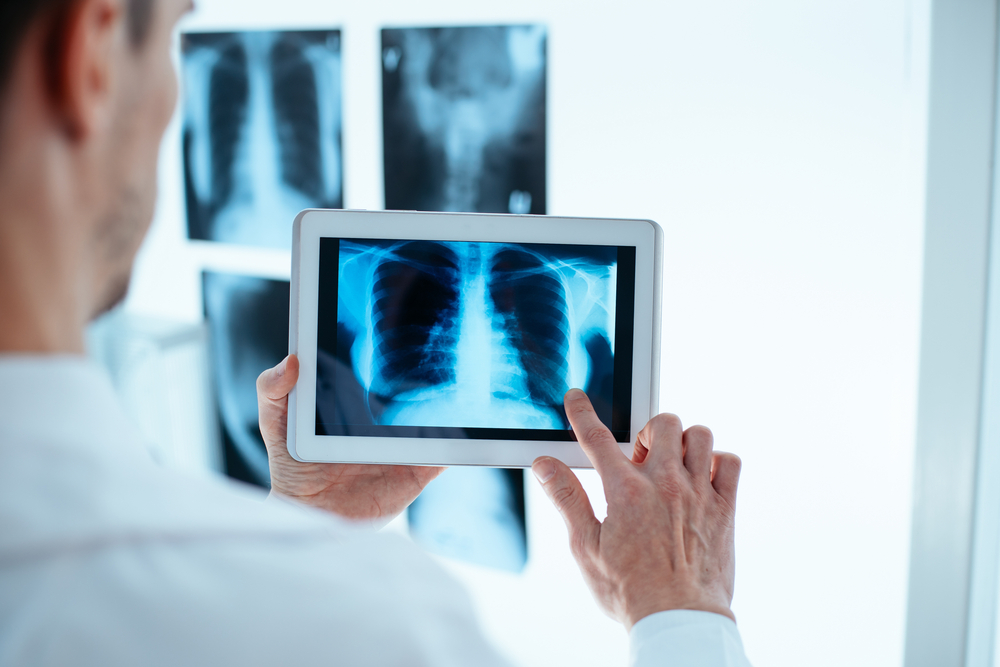
\includegraphics[width=0.55\linewidth]{img/X-ray_results.png}
            % \caption{Adversarial Attack in Transportation}
            % \label{fig:StopToGo}
        \end{figure}
    \end{columns}
\end{frame}

% %------------------------------------------------
\begin{frame}{Where does Transfer Learning Attack occur?}
    \begin{itemize}
        \item Transfer Learning Attacks can target multiple critical domains where AI and machine learning models are widely used.
    \end{itemize}

    \begin{columns}
        \column{0.5\textwidth}
        \begin{itemize}
            \item \textbf{\large Finance:}
            \begin{itemize}
                \item Exploiting fraud detection models by injecting poisoned data.
                % \item Example: Approving illegitimate transactions.
            \end{itemize}
            \begin{figure}[h]
                \centering
                
\includegraphics[width=0.7\linewidth]{img/Approving_illegitimate_transactions.png}
                % \caption{Enter Caption}
                % \label{fig:enter-label}
            \end{figure}
        \end{itemize}

        \column{0.5\textwidth}
        \begin{itemize}
            \item \textbf{\large Security:}
            \begin{itemize}
                \item Circumventing intrusion detection systems.
                % \item Example: Using adversarial inputs to bypass firewall defenses.
            \end{itemize}
            \begin{figure}
                \centering
                
\includegraphics[width=0.7\linewidth]{img/firewall bypassing.png}
                % \caption{Enter Caption}
                % \label{fig:enter-label}
            \end{figure}
        \end{itemize}
    \end{columns}
\end{frame}

% %------------------------------------------------
\begin{frame}{Who: Who attacks and who are the victims?}
    \begin{columns}
        % Left Column: The Attackers
        \column{0.5\textwidth}
        \textbf{\large The Attackers:}
        \begin{itemize}
            \item \textbf{Characteristics:}
            \begin{itemize}
                \item Individuals or organizations with diverse motivations.
                \item Can range from malicious hackers to competing entities.
            \end{itemize}
            \item \textbf{Goals:}
            \begin{itemize}
                \item \textbf{Disrupt operations:}
                \begin{itemize}
                    \item Cause technological or financial damage.
                \end{itemize}
                \item \textbf{Steal sensitive data:}
                \begin{itemize}
                    \item Misuse or sell confidential information obtained from attacked models.
                \end{itemize}
            \end{iuutemize}
        \end{itemize}

        % Right Column: The Victims
        \column{0.5\textwidth}
        \begin{itemize}
            \begin{figure}
                \centering
                
\includegraphics[width=1\linewidth]{img/Attacker.png}
                % \caption{The Attackers}
                \label{fig:The_Attacker}
            \end{figure}
        \end{itemize}
    \end{columns}
\end{frame}
% %------------------------------------------------
\begin{frame}{Who: Who attacks and who are the victims?}
    \begin{columns}
        % Left Column: The Attackers
        \column{0.5\textwidth}
        \begin{itemize}
            \begin{figure}
                \centering
                
\includegraphics[width=1\linewidth]{img/The_Victim.png}
                %\caption{Enter Caption}
                %\label{fig:enter-label}
            \end{figure}
        \end{itemize}

        % Right Column: The Victims
        \column{0.5\textwidth}
        \textbf{\large The Victims:}
        \begin{itemize}
            \item \textbf{Characteristics:}
            \begin{itemize}
                \item Companies using Transfer Learning models.
                \item End-users who rely on these systems for critical tasks.
            \end{itemize}
            \item \textbf{Impacts:}
            \begin{itemize}
                \item Loss of operational trust.
                \item Exposure to legal, financial, and reputational risks.
                \item Potential harm to users depending on critical applications (e.g., healthcare, self-driving cars).
            \end{itemize}
        \end{itemize}
    \end{columns}
\end{frame}
% %------------------------------------------------
\begin{frame}{Consequences of Transfer Learning Attack}
    \begin{itemize}
        \item \textbf{Key Examples:}
        \begin{itemize}
            \item \textbf{Misclassification:} 
            \begin{itemize}
                \item Attacks like adversarial examples can cause models to misclassify objects, leading to system errors.
                %\item Example: Facial recognition misidentifying an intruder as a legitimate person.
            \end{itemize}
            \item \textbf{Data Exfiltration:} 
            \begin{itemize}
                \item Attackers may extract sensitive information from training datasets, such as personal, financial, or medical data.
                %\item Example: White-box attacks extracting patient identities from diagnostic models.
            \end{itemize}
            \item \textbf{Asset Loss:} 
            \begin{itemize}
                \item Financial losses due to manipulated models or incorrect predictions.
                %\item Example: Market prediction models leading to poor investment decisions.
            \end{itemize}
        \end{itemize}
    \end{itemize}

    \begin{figure}[h]
        \centering
        \begin{minipage}{0.4\textwidth} % Adjust width to fit the image
            \centering
            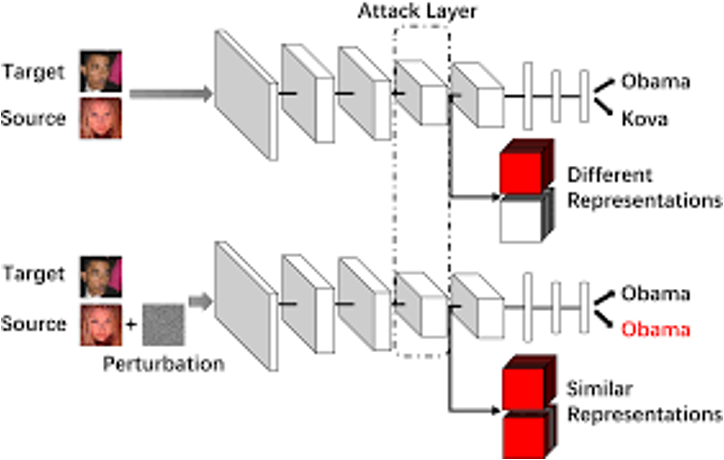
\includegraphics[width=\textwidth]{img/consequence.png} % Replace with actual image path
        \end{minipage}
        \begin{minipage}{0.35\textwidth} % Adjust width as needed
            \caption{Examples of the Consequences of Transfer Learning Attack.}
            \label{fig:transfer-attack}
        \end{minipage}%
    \end{figure}
\end{frame}

% %------------------------------------------------
\begin{frame}{How to Prevent Transfer Learning Attacks?}
    \begin{columns}
        \column{0.5\textwidth}
        \textbf{Key Preventative Measures:}
        \begin{itemize}
            \item Secure Training Data
            \item Model Isolation
            \item Knowledge Distillation
            \item Differential Privacy
            \item Adversarial Training
        \end{itemize}
    
        \column{0.5\textwidth}
        \textbf{Additional Techniques:}
        \begin{itemize}
            \item Data Augmentation
            \item Ensemble Methods
            \item Post-processing and anomaly detection
        \end{itemize}
    \end{columns}
    \begin{figure}[h]
        \centering
        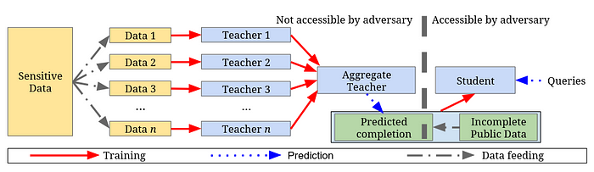
\includegraphics[width=0.53\textwidth]{img/how-to-prevent.png}
        \label{fig:how-to-prevent}
        \caption{Differential privacy as a protection to Transfer Learning attacks}
    \end{figure}
\end{frame}



% \begin{frame}
% 	\frametitle{Text paragraph}
%     Lorem ipsum dolor sit amet, consectetur adipiscing elit. Nullam ipsum velit, cursus quis ligula eu, malesuada aliquet massa. Quisque non convallis felis, a auctor eros. Etiam sit amet turpis a sapien pulvinar malesuada quis quis nisi. Quisque scelerisque volutpat ligula vel mollis. Nam sit amet tristique erat, sit amet cursus mi. 
% \end{frame}

% %------------------------------------------------

% \begin{frame}
% 	\frametitle{Text with enumerate }
%      Lorem ipsum dolor sit amet, consectetur adipiscing elit:
%     \begin{enumerate}
%         \item Lorem ipsum dolor sit amet.
%         \item Lorem ipsum dolor sit amet.
%     \end{enumerate}
	
% \end{frame}

% %------------------------------------------------

% \begin{frame}
% 	\frametitle{Text with itemize}
%      Lorem ipsum dolor sit amet, consectetur adipiscing elit:
%     \begin{itemize}
%         \item Lorem ipsum dolor sit amet.
%         \item Lorem ipsum dolor sit amet.
%     \end{itemize}
	
% \end{frame}

%------------------------------------------------



\section{Experiments}
%------------------------------------------------

% \begin{frame}{Single images}
%    \begin{figure}[h]
%        \centering
%        
\includegraphics[width=0.7\textwidth]{img/logo_v2.png}
%        \caption{Slide with single images}
%        \label{fig:sing_image}
%    \end{figure}
% \end{frame}

% %------------------------------------------------

% \begin{frame}{Single image with itemize}
%      Lorem ipsum dolor sit amet, consectetur adipiscing elit:
%     \begin{enumerate}
%         \item Lorem ipsum dolor sit amet.
%         \item Lorem ipsum dolor sit amet.
%     \end{enumerate}
    
%    \begin{figure}[h]
%        \centering
%        
\includegraphics[width=0.7\textwidth]{img/logo_v2.png}
%        \caption{Slide with single images}
%        \label{fig:sing_image}
%    \end{figure}
% \end{frame}

%------------------------------------------------
\begin{frame}{Methodology}

\begin{columns}

\column{0.3\textwidth}
 \footnotesize
    \begin{thebibliography}{99}
        \bibitem{autorlivro} Zhang, Yinghua, et al. "Two sides of the same coin: White-box and black-box attacks for transfer learning." Proceedings of the 26th ACM SIGKDD international conference on knowledge discovery \& data mining. 2020.

    \end{thebibliography}

\column{0.7\textwidth}
    \begin{figure}
        \begin{subfigure}{0.9\textwidth}
            \centering
            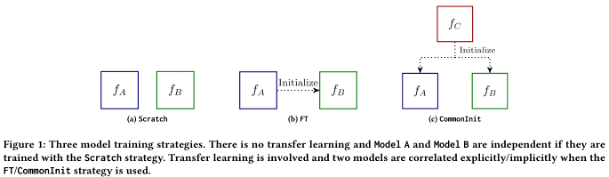
\includegraphics[scale=0.55]{img/exper-1.png}
     
            \label{fig:sub-figure-url-1}
        \end{subfigure} \\
        \begin{subfigure}{0.9\textwidth}
            \centering
            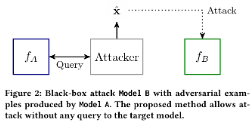
\includegraphics[scale=0.55]{img/exper-2.png}
    
            \label{fig:sub-figure-url-2}
        \end{subfigure}
        \label{fig:example-subfigure}
    \end{figure}
    \begin{itemize}
        \item Datasets: MNIST (M), USPS (U), SVHN (S), SynDigits (Syn), CIFAR10, STL10, ImageNet32
    \end{itemize}
\end{columns}

\end{frame}

%------------------------------------------------
\begin{frame}{White-box Attack Experiment}
\begin{columns}[T]
    \column{0.4\textwidth}
        \begin{itemize}
            \item \textbf{Goal}: Assess robustness to FGSM attacks.
            \item \textbf{Method}: Compare Scratch vs. Fine-tuning models under various noise levels.
            \item \textbf{Result}:
            \begin{itemize}
                \item Fine-tuning significantly improves accuracy and robustness.
                \item Example: Accuracy increases from 50.86\% -> 84.96\% at $\epsilon = 0.125$.
            \end{itemize}
            % \item \textbf{Conclusion}: Fine-tuning enhances both performance and security.
        \end{itemize}

    \column{0.6\textwidth}
       \begin{figure}[h]
           \centering
           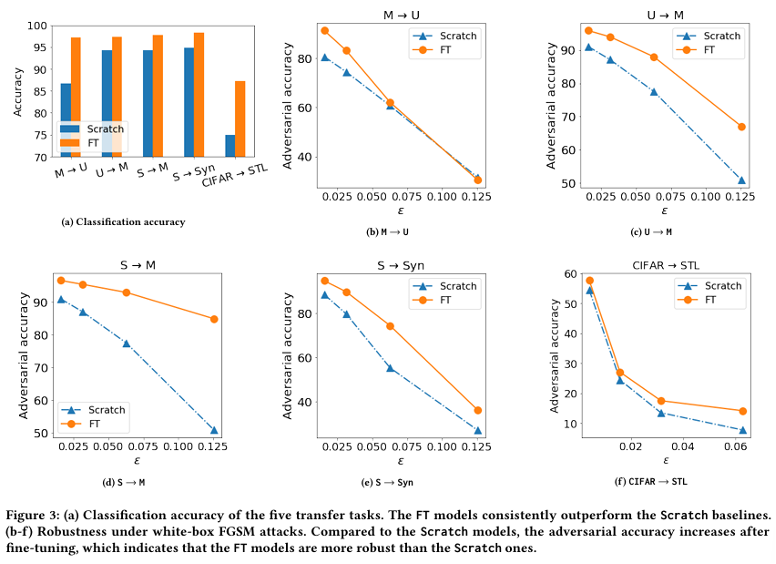
\includegraphics[scale=0.7]{img/white-box.png}
           \label{fig:what-is}
       \end{figure}
    \end{columns}
\end{frame}
%------------------------------------------------
\begin{frame}{Black-box Attack Experiment}
\begin{columns}[T]
    \column{0.6\textwidth}
       \begin{figure}[h]
           \centering
           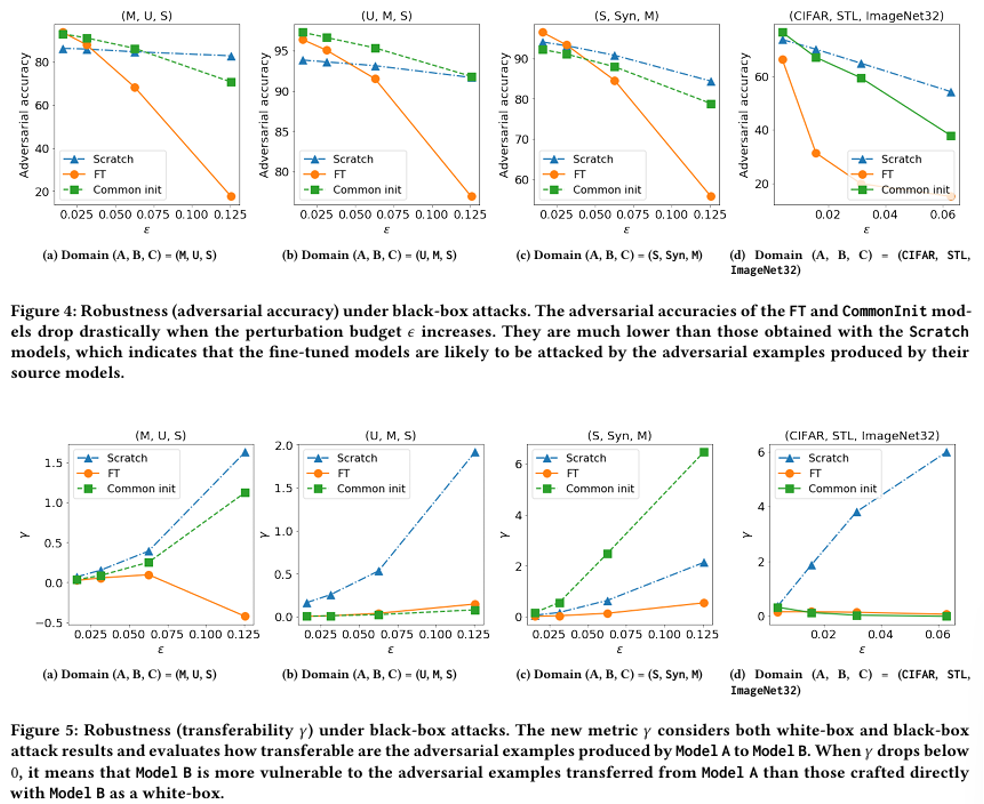
\includegraphics[scale=0.5]{img/black-box.png}
           \label{fig:black-box}
       \end{figure}
    \column{0.4\textwidth}
        \begin{itemize}
            \item \textbf{Goal}: Evaluate transferability of adversarial examples.
            \item \textbf{Method}: Attack model B using adversarial examples from model A.
            \item \textbf{Result}:
            \begin{itemize}
                \item Fine-tuned models are more vulnerable to transferred attacks.
                \item Example: Accuracy drops from 87.43\% -> 65.32\% (FGSM).
            \end{itemize}
            % \item \textbf{Conclusion}: Fine-tuning improves performance but increases attack susceptibility.
        \end{itemize}
\end{columns}
\end{frame}

%------------------------------------------------

\section{Conclusions}

%------------------------------------------------
\begin{frame}{Author's Conclusion}
\setstretch{1.5} % Set line spacing to 1.5
    \begin{itemize}
        \item \textbf{Fine-tuning improves robustness:}
        \begin{itemize}
            \item Fine-tuning models enhance performance and security under white-box FGSM attacks.
        \end{itemize}
        \item \textbf{Risks of Fine-tuning:}
        \begin{itemize}
            \item Fine-tuned models are more vulnerable to adversarial examples from their source models.
            \item Black-box attacks demonstrate increased risks when transfer learning is applied.
        \end{itemize}
        \item \textbf{Findings' Implication:}
        \begin{itemize}
            \item Highlights a trade-off between improved performance and susceptibility to attacks.
        \end{itemize}
    \end{itemize}
\end{frame}

%------------------------------------------------
\begin{frame}{Author's Conclusion}
\setstretch{1.5} % Set line spacing to 1.5
    \begin{itemize}
        \item \textbf{New Metrics:}
        \begin{itemize}
            \item Introduced a metric to evaluate the transferability of adversarial attacks.
        \end{itemize}
        \item \textbf{Future Implications:}
        \begin{itemize}
            \item Findings provide insights for designing transfer learning models that are robust and effective.
            \item Encourages further research into adversarial robustness in transfer learning.
        \end{itemize}
        \item \textbf{Call to Action:}
        \begin{itemize}
            \item Developers need to carefully consider potential risks in fine-tuned systems.
        \end{itemize}
    \end{itemize}
\end{frame}

%------------------------------------------------
\begin{frame}{Contributions of the Paper}
\setstretch{1.5} % Set line spacing to 1.5
    \begin{itemize}
        \item \textbf{Comprehensive Experiments:}
        \begin{itemize}
            \item Evaluated robustness of fine-tuned models under both white-box and black-box attacks.
        \end{itemize}
        \item \textbf{Novel Insights:}
        \begin{itemize}
            \item Demonstrated trade-offs between performance and security in transfer learning.
        \end{itemize}
        \item \textbf{New Evaluation Metrics:}
        \begin{itemize}
            \item Proposed a metric to assess the transferability of adversarial examples.
        \end{itemize}
        \item \textbf{Practical Implications:}
        \begin{itemize}
            \item Findings emphasize the importance of adversarial training and robust model design.
        \end{itemize}
    \end{itemize}
\end{frame}


% \begin{frame}{Equation}
%     Navier-Stokes Equations Expanded Form (3D):
%     \footnotesize
%         \begin{align*}
%             \rho\left(\frac{\partial u}{\partial t} + u\frac{\partial u}{\partial x} + v\frac{\partial u}{\partial y} + w\frac{\partial u}{\partial z}\right) &= -\frac{\partial p}{\partial x} + \mu\left(\frac{\partial^2 u}{\partial x^2} + \frac{\partial^2 u}{\partial y^2} + \frac{\partial^2 u}{\partial z^2}\right) + f_x \\[0.3cm]
%             \rho\left(\frac{\partial v}{\partial t} + u\frac{\partial v}{\partial x} + v\frac{\partial v}{\partial y} + w\frac{\partial v}{\partial z}\right) &= -\frac{\partial p}{\partial y} + \mu\left(\frac{\partial^2 v}{\partial x^2} + \frac{\partial^2 v}{\partial y^2} + \frac{\partial^2 v}{\partial z^2}\right) + f_y \\[0.3cm]
%             \rho\left(\frac{\partial w}{\partial t} + u\frac{\partial w}{\partial x} + v\frac{\partial w}{\partial y} + w\frac{\partial w}{\partial z}\right) &= -\frac{\partial p}{\partial z} + \mu\left(\frac{\partial^2 w}{\partial x^2} + \frac{\partial^2 w}{\partial y^2} + \frac{\partial^2 w}{\partial z^2}\right) + f_z
%         \end{align*}
        
%     where $\mathbf{v} = (u,v,w)$ is the velocity field, $p$ is the pressure, $\rho$ is the density, $\mu$ is the dynamic viscosity, and $\mathbf{f}$ represents external forces.
% \end{frame}

% %------------------------------------------------

% \begin{frame}[fragile]
%     \frametitle{Python}
    
%     \begin{python}
% def calcular_dobro(x):
%     """Retorna o dobro do número"""
%     return 2 * x

% # Testando a função
% numero = 5
% resultado = calcular_dobro(numero)
% print(f"O dobro de {numero} é {resultado}")
%     \end{python}
% \end{frame}

% %------------------------------------------------
% \begin{frame}[fragile]
%     \frametitle{Java}
    
%     \begin{java}
% public class Exemplo {
%     public static void main(String[] args) {
%         int numero = 5;
%         int dobro = 2 * numero;
        
%         System.out.println("O dobro de " + numero +
%                          " eh " + dobro);
%     }
% }
%     \end{java}
% \end{frame}
% %------------------------------------------------

% \section{Specific feature}
%------------------------------------------------
\begin{frame}
\frametitle{Slide with highligh text}

In this slide, some important text will be
\alert{highlighted} because it's important.
Please, don't abuse it.

\begin{block}{Remark}
Sample text
\end{block}

\begin{alertblock}{Important theorem}
Sample text in red box
\end{alertblock}

\begin{examples}
Sample text in green box. The title of the block is ``Examples".
\end{examples}
\end{frame}
%------------------------------------------------
\begin{frame}
\frametitle{Slide with transition}
In this slide \pause

the text will be partially visible \pause

And finally everything will be there
\end{frame}

%------------------------------------------------

\begin{frame}
\frametitle{Two-column slide}

\begin{columns}

\column{0.5\textwidth}
This is a text in first column.
$$E=mc^2$$
\begin{itemize}
\item First item
\item Second item
\end{itemize}

\column{0.5\textwidth}
This text will be in the second column
and on a second tought this is a nice looking
layout in some cases.
   \begin{figure}[h]
       \centering
       
\includegraphics[scale=0.1]{img/logo_v2.png}
       \caption{Image on right column}
       \label{fig:right_side}
   \end{figure}
\end{columns}
\end{frame}

%------------------------------------------------
% \section{Conclution} % Seções são adicionadas para organizar sua apresentação em blocos discretos, todas as seções e subseções são automaticamente exibidas no índice como uma visão geral da apresentação, mas NÃO são exibidas como slides separados.

\begin{frame}{References}
    \footnotesize
    \begin{thebibliography}{99}
        \bibitem{autorlivro} SOBRENOME, Nome do autor, \textit{Título do livro}, Edição, Editora, Ano de publicação, Local de publicação.
        \bibitem{autorartigo} SOBRENOME, Nome do autor, \textit{Título do artigo}, Nome do periódico, Ano de publicação, Volume(Número), pp. Páginas, Local de publicação.
        \bibitem{autorTese} SOBRENOME, Nome do autor, \textit{Título da tese/dissertação}, Nome da instituição, Tese (ou Dissertação), Ano de publicação, Local de publicação.
    \end{thebibliography}
\end{frame}



%----------------------------------------------------------------------------------------
%	CLOSING SLIDE
%----------------------------------------------------------------------------------------

\begin{frame}[plain] % The optional argument 'plain' hides the headline and footline
	\begin{center}
		{\Huge Thanks for your attention}
            
	\end{center}
\end{frame}

%----------------------------------------------------------------------------------------

\end{document} 